\documentclass[a4paper]{article}
\usepackage[utf8]{inputenc}
\usepackage[italian]{babel}
\usepackage[hidelinks]{hyperref}
\usepackage{graphicx}
\usepackage{pdfpages}
\usepackage{subfig}
\usepackage{float}
\usepackage{listings}
\usepackage{xcolor}
\definecolor{codegreen}{rgb}{0,0.6,0}
\definecolor{backcolour}{rgb}{0.95,0.95,0.95}
\definecolor{codepurple}{rgb}{0.58,0,0.82}
\lstdefinestyle{style}{
    backgroundcolor=\color{backcolour},   
    commentstyle=\color{codegreen},
    keywordstyle=\color{magenta},
    stringstyle=\color{codepurple},
    basicstyle=\ttfamily\footnotesize,
    breakatwhitespace=false,         
    breaklines=true,                 
    captionpos=b,                    
    keepspaces=true,                 
    numbers=left,                    
    numbersep=5pt,                  
    showspaces=false,                
    showstringspaces=false,
    showtabs=false,                  
    tabsize=2
}
\lstset{style=style}
\title{
	Assignment 5 \\
	\large Visual Information Processing and Management}
\author{Davide Costantini, 856114}
\date{27 novembre 2025}
\begin{document}
	\maketitle
	\newpage
	\section{Bag of Words}
    Sono state effettuate le seguenti modifiche:
    \begin{itemize}
        \item featStep = 15: è lo spazio che viene lasciato tra i keypoint, ovvero la densità della griglia. È stato
              ridotto in modo da prelevare un maggior numero di keypoint.
        \item imSize = 750: è la dimensione che devono avere le immagini nel momento in cui vengono prelevati i
              keypoint.
        \item nIm4Training = 60: sono il numero di immagini (per classe) utilizzate per il training. È stato ridotto per
              avere 10 immagini da usare per la validazione e mantenere 30 immagini per il test.
        \item K = 150: è il numero di cluster utilizzati dal k-means, che nel caso di Bag of Words coincidono con le
              parole. È stato alzato leggermente rispetto al valore originale per avere più parole, e quindi una
              migliore rappresentazione delle immagini.
    \end{itemize}
    \begin{table}[H]
        \begin{center}
            \begin{tabular}{l|c|c|c|c}
                            & \textbf{featStep} & \textbf{imsize}   & \textbf{K}    & \textbf{Accuracy} \\
                \hline
                Laboratorio & 30                & 500               & 100           & 48.67\%              \\
                Assignment  & 15                & 750               & 150           & 64.33\%           \\
            \end{tabular}
        \end{center}
    \end{table}
    \begin{figure}[H]
        \centering
        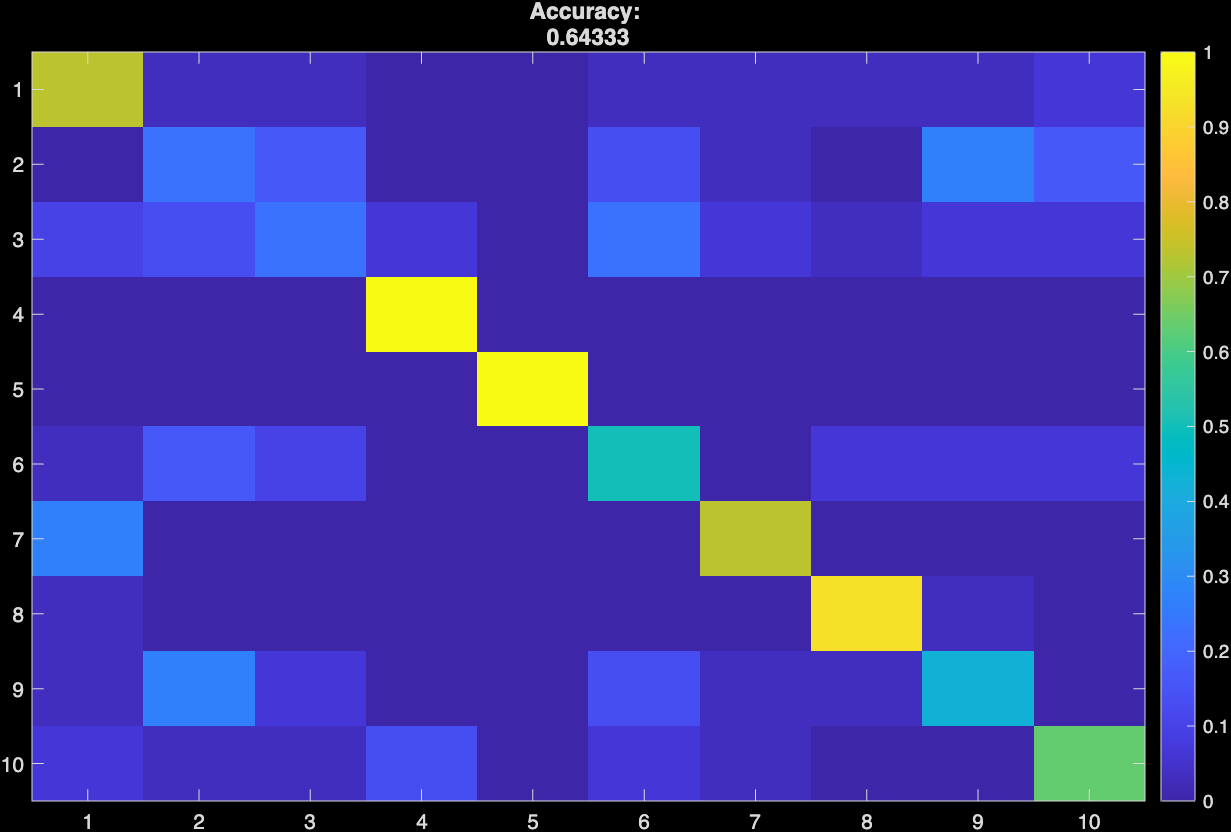
\includegraphics[width=\columnwidth]{images/confusionMatrix}
        \caption{Matrice di confusione}
    \end{figure}
    \newpage
	\section{Codice}
    \lstinputlisting[language=Matlab]{../bow_assignment.m}
\end{document}
